\chapter{Decision making}
All the problems you have solved so far have been problems with a \textit{straight-line} logic pattern \ie\ you followed a sequence of steps (defining variables, performing calculations, displaying results) that flowed directly from one step to another. Decision making is an important concept in programming and allows you to control which parts of your code should execute depending on certain conditions. This flow of control in your program can be performed by branching with \mcode{if} and \mcode{else} statements, which will be discussed in this chapter, or looping, which will be discussed in Chapter~\ref{ch:loops}. 

\section{Relational and logical operations}
Relational and logical operators are used in branching and looping to help make decisions. The result of using a relational or logical operator will always be either true, given by a \mcode{1}, or false, given by a \mcode{0}. Tables~\ref{tab:relational_ops}--\ref{tab:logical_ops} list the most common relational and logical operators in \mlab.

\begin{table}[h]
	\caption{Relational operators}
	\label{tab:relational_ops}
	\myfloatalign
	\begin{tabular}{lcc}\toprule
	\spacedlowsmallcaps{Operator} & \spacedlowsmallcaps{Mathematical symbol} & \spacedlowsmallcaps{\mlab symbol} \\ \midrule
	Equal & $=$ & $==$ \\
	Not equal & $\neq$ & $\sim=$ \\
	Less than & $<$ & $<$ \\
	Greater than & $>$ & $>$ \\
	Less than or equal & $\leq$ & $<=$ \\
	Greater than or equal & $\geq$ & $>=$\\
	\bottomrule
	\end{tabular}
\end{table}

\begin{table}[h]
	\caption{Logical operators}
	\label{tab:logical_ops}
	\myfloatalign
	\begin{tabular}{lcc}\toprule
	\spacedlowsmallcaps{Operator} & \spacedlowsmallcaps{Mathematical symbol} & \spacedlowsmallcaps{\mlab symbol} \\ \midrule
	And & AND & $\&$ \\
	Or & OR & $|$ \\
	Not & NOT & $\sim$ \\
	\bottomrule
	\end{tabular}
\end{table}
\newpage
Listings~\ref{lst:simple_relational_ops} presents a simple example of using relational operators.
\begin{lstlisting}[caption={Simple relational operators},label=lst:simple_relational_ops]
>> x = 5;
>> y = 10;
>> x<y
ans =
	 1
>> x>y
ans =
	 0
\end{lstlisting}
\subsubsection{Comments:}
\begin{itemize}
\item Lines 3 and 6 are called logical expression because the result can only be either true, represented by \mcode{1}, or false, represented by \mcode{0}.
\end{itemize}
Listings~\ref{lst:relational_ops}--\ref{lst:logical_ops} present more examples of using relational and logical operators.
\begin{lstlisting}[caption={Relational operators},label=lst:relational_ops]
>> x = [1 5 3 7];
>> y = [0 2 8 7];
>> k = x<y
k =
	0    0    1    0
>> k = x<=y
k =
	0    0    1    1
>> k = x>y
k =
	1    1    0    0
>> k = x>=y
k =
	1    1    0    1
>> k = x==y
k =
	0    0    0    1
>> k = x~=y
k =
	1    1    1    0
\end{lstlisting}

\begin{lstlisting}[caption={Logical operators},label=lst:logical_ops]
>> x = [1 5 3 7];
>> y = [0 2 8 7];
>> k = (x>y) & (x>4)
k =
	0    1    0    0
>> k = (x>y) | (x>4)
k =
	1    1    0    1
>> k = ~((x>y) | (x>4))
k =
	0    0    1    0
\end{lstlisting}

\subsubsection{Comments:}
\begin{itemize}
\item The relational and logical operators are used to compare, element-by-element, the vectors \mcode{x} and \mcode{y}.
\item The result of each comparison is a logical vector \ie\ \mcode{k} only contains 1's and 0's (corresponding to true or false).
\end{itemize}

\addtolength{\parindent}{-4mm}
\fcolorbox{myborderblue}{myblue}{%
\begin{minipage}{\linewidth}
\begin{minipage}{6mm}

\includegraphics[scale=0.03]{Graphics/General/help_icon}
\end{minipage}
\textit{Single and double equals signs} \\
The difference between \mcode{=} and \mcode{==} is often misunderstood. A single equals sign is used to assign a value to a variable \eg\ \mcode{x=5}. A double equals sign is used to test whether a variable is equal to given value \eg\ \mcode{my_test=(x==5)} means test if \mcode{x} is equal to 5, and if so assign the value \mcode{1} (true) to \mcode{my_test}.
\end{minipage}%
}\\
\addtolength{\parindent}{4mm}
\vspace{5mm}

%%%%%%%%%%%%%%%%%%%%%%%%%%%%%%%%%%%%%%%%%%%%%%
% Self Test Exercise: Relational and logical operators
%%%%%%%%%%%%%%%%%%%%%%%%%%%%%%%%%%%%%%%%%%%%%%
\addtolength{\parindent}{-4mm}
\begin{minipage}{\linewidth}
\begin{minipage}{6mm}

\includegraphics[scale=0.035]{Graphics/General/exercise_icon}
\end{minipage}
\textit{Self Test Exercise: Relational operators and logical}
\end{minipage}
\addtolength{\parindent}{4mm}
\begin{enumerate}
\item \footnote[2]{Question adapted from \gilatbook}Evaluate the following expressions without using \mlab. Check your answer with \mlab.
\begin{enumerate}
\item $14 > 15 / 3$
\item $y = 8 / 2 < 5 \times 3 + 1 > 9$
\item $y = 8/(2 < 5) \times 3 + (1 > 9)$
\item $2 + 4 \times 3  \sim = 60 / 4 - 1$
\end{enumerate}

\item \footnotemark[2]Given: \mcode{a=4}, \mcode{b=7}. Evaluate the following expressions without using \mlab. Check your answer with \mlab.
\begin{enumerate}
\item $y = a + b  >= a\times b$
\item $y = a + (b  >= a) \times b$
\item $y = b - a < a < a/b$
\end{enumerate}

\item \footnotemark[2]Given: \mcode{v=[4 -2 -1 5 0 1 -3 8 2]}, and \mcode{w=[0 2 1 -1 0 -2 4 3 2]}. Evaluate the following expressions without using \mlab. Check your answer with \mlab.
\begin{enumerate}
\item $v  <= w$
\item $w = v$
\item $v < w + v$
\item $(v < w) + v$
\end{enumerate}
\end{enumerate}

\section{The if-else statement}
The \mcode{if}, \mcode{else}, and \mcode{elseif} statements in \mlab provide methods of controlling which parts of your code should execute based on whether certain conditions are true or false. The syntax of the simplest form of an \mcode{if} statement is given in Listing~\ref{lst:if_structure}.
\begin{lstlisting}[caption={Syntax of an \mcode{if} statement},label=lst:if_structure]
if **logical_expression**
	**statements**
end
\end{lstlisting}

\subsubsection{Comments:}
\begin{itemize}
\item Line 1 contains the \mcode{if} command, followed by an expression which must return true or false.
\item Line 2 contains the body of the \mcode{if} statement which can be a command or series of commands that will be executed if the logical expression returns \mcode{true}.
\item Line 3 contains the \mcode{end} command which must always be used to close the \mcode{if} statement.
\item If the logical expression returns true \mlab will execute the statements enclosed between \mcode{if} and \mcode{end}. If the logical expression returns false \mlab will skip the statements enclosed between \mcode{if} and \mcode{end} and proceed with any following code.
\end{itemize}
Listing~\ref{lst:basic_if} presents a very simple example of using an \mcode{if} statement to test if a user has entered a number greater than 10.

\newpage
\lstinputlisting[caption={\textit{basic\_if.m} - Script to show simple if statement},label=lst:basic_if]{MATLAB-code/Document/basic_if.m}

\subsubsection{Comments:}
\begin{itemize}
\item On Line 12 the \mcode{input} command is used, which prompts the user for input with the request \mcode{Enter a number: } and assigns the number entered to the variable \mcode{x}.
\item On Line 13 an \mcode{if} statement is used with the logical expression \mcode{x>10}. If this expression is true then the text \mcode{Your number is greater than 10} is displayed, otherwise if the expression is false nothing is executed.
\end{itemize}

The \mcode{else} and \mcode{elseif} commands can be used to apply further conditions to the \mcode{if} statement. Listing~\ref{lst:if_else_elseif_structure} presents the syntax of these commands.
\begin{lstlisting}[caption={Syntax of an \mcode{if} statement with \mcode{else} and \mcode{elseif}},label=lst:if_else_elseif_structure]
if **logical_expression**
	**statements**
elseif **logical_expression**
	**statements**
else
	**statements**
end
\end{lstlisting}

\subsubsection{Comments:}
\begin{itemize}
\item On Line 3 the logical expression associated with the \mcode{elseif} command will only be evaluated if the preceding logical expression associated with the \mcode{if} command returns false.
\item Notice that the \mcode{else} command on Line 5 has no associated logical expression. The statements following the \mcode{else} command will only be executed if all the logical expressions for the preceding \mcode{elseif} and \mcode{if} commands return false.
\end{itemize}
Listing~\ref{lst:if_else_elseif_example} presents a simple of example of decision making using the \mcode{if}, \mcode{else}, and \mcode{elseif} functions. Copy and paste the example into a new script file, and run it to see the results for yourself.

\lstinputlisting[caption={\textit{number\_test.m} - Script to test sign and magnitude of numbers},label=lst:if_else_elseif_example]{MATLAB-code/Document/number_test.m}

\subsubsection{Comments:}
\begin{itemize}
\item On Line 12 the \mcode{input} command is used, which prompts the user for input with the request \mcode{Enter a number: } and assigns the number entered to the variable \mcode{x}.
\item On Lines 14, 16, and 18 the \mcode{disp} command is used, which simply displays text to the Command Window.
\end{itemize}

%%%%%%%%%%%%%%%%%%%%%%%%%%%%%%%%%%%%%%%%%%%%%%
% Screencast: The if-else statement
%%%%%%%%%%%%%%%%%%%%%%%%%%%%%%%%%%%%%%%%%%%%%%
\addtolength{\parindent}{-4mm}
\fcolorbox{myborderblue}{myblue}{%
\begin{minipage}{\linewidth}
\setcounter{mpfootnote}{\value{footnote}}
\renewcommand{\thempfootnote}{\fnsymbol{mpfootnote}}
\begin{minipage}{6mm}

\includegraphics[scale=0.03]{Graphics/General/screencast_icon}
\end{minipage}
\href{http://www.eng.ed.ac.uk/teaching/courses/matlab/unit04/if-else-statement.shtml}{\screencast{The if-else statement}}\\
(http://www.eng.ed.ac.uk/teaching/courses/matlab/unit04/if-else-statement.shtml)\\ \\
The following example is solved in the screencast:\\ \\
\textit{Water level in a water tower\footnote[2]{Question adapted from \gilatbook}}\\
The tank in a water tower has the geometry shown in Figure~\ref{fig:water-tower} (the lower part is a cylinder and the upper part is an inverted frustum cone). Inside the tank there is a float that indicates the level of the water. Write a user-defined function that determines the volume of water in the tank from the position (height) of the float. The volume for the cylindrical section of the tank is given by:
\begin{equation*}
V = \pi \cdot 12.5^2 \cdot h
\end{equation*}
The volume for the cylindrical and conical sections of the tank is given by:
\begin{align*}
V &= \pi \cdot 12.5^2 \cdot 19 + \frac{1}{3}\pi (h - 19)(12.5^2 + 12.5r_h + {r_h}^2), \\
\textrm{where} \quad r_h &= 12.5 + \frac{10.5}{14} (h - 19)
\end{align*}
[$h = 8~m$, $V = 3927~m^3$; $h = 25.7~m$, $V = 14115~m^3$]
\end{minipage}%
}\\
\addtolength{\parindent}{4mm}
\begin{figure}[h]
	\myfloatalign
	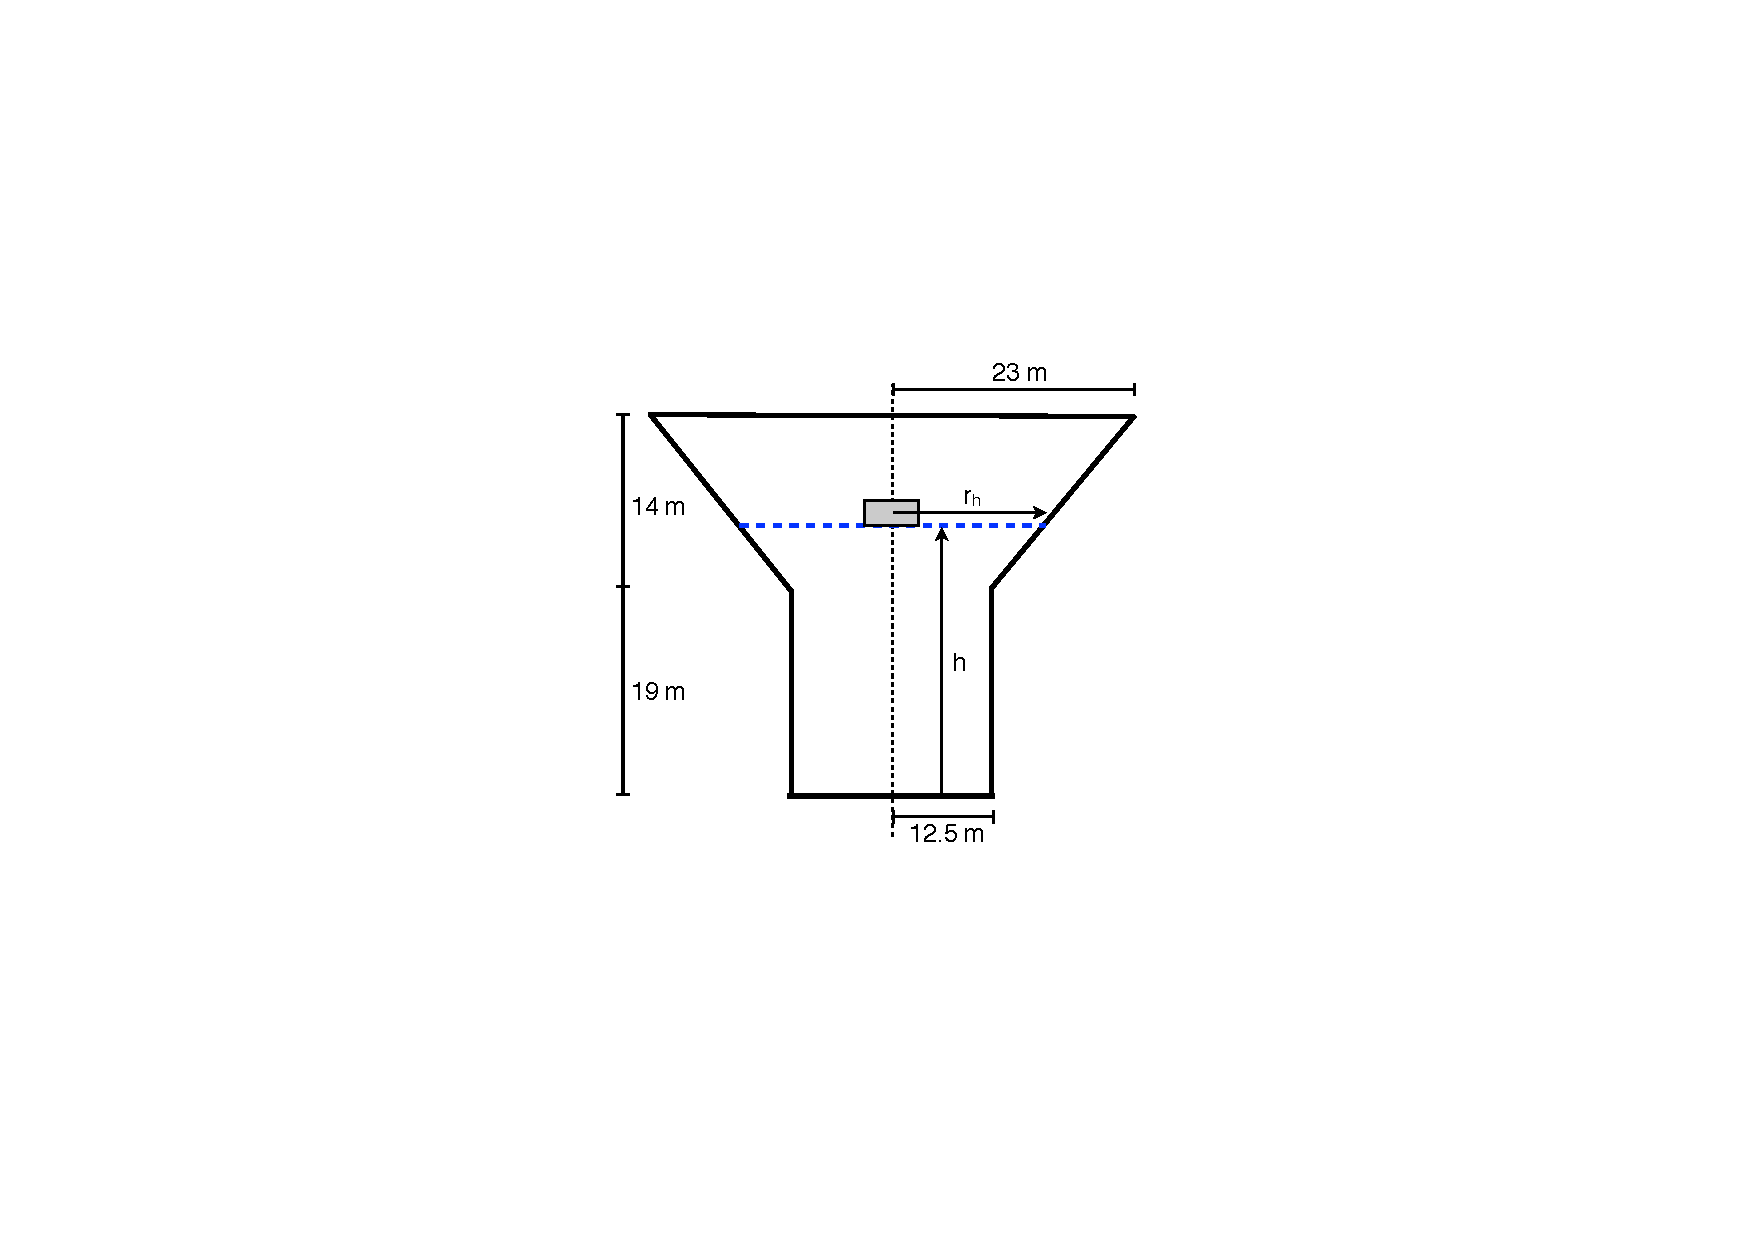
\includegraphics[width=0.65\linewidth]{Graphics/Additional-Ex/water-tower}
	\caption{Water level in a water tower}
	\label{fig:water-tower}
\end{figure}

\newpage
%%%%%%%%%%%%%%%%%%%%%%%%%%%%%%%%%%%%%%%%%%%%%%
% Self Test Exercise: The if-else statement
%%%%%%%%%%%%%%%%%%%%%%%%%%%%%%%%%%%%%%%%%%%%%%
\addtolength{\parindent}{-4mm}
\begin{minipage}{\linewidth}
\begin{minipage}{6mm}

\includegraphics[scale=0.035]{Graphics/General/exercise_icon}
\end{minipage}
\textit{Self Test Exercise: The if-else statement}
\end{minipage}
\addtolength{\parindent}{4mm}
\\ Evaluate the following expressions without using \mlab.
\begin{enumerate}
\item Which of the following shows a correct \mcode{if}, \mcode{else} statement?
\begin{enumerate}
\item . \vspace{-2mm} 
\begin{lstlisting}
a = input('a? ')
If a < 0
	disp('a is negative')
ELSEIF a == 0
	disp('a is equal to zero')
Else
	disp('a is positive')
END
\end{lstlisting}

\item . \vspace{-2mm}
\begin{lstlisting}
a = input('a? ')
if a < 0
	disp('a is negative')
elseif a = 0
	disp('a is equal to zero')
else
	disp('a is positive')
end
\end{lstlisting}

\item . \vspace{-2mm}
\begin{lstlisting}
a = input('a? ')
if a < 0
	disp('a is negative')
elseif a == 0
	disp('a is equal to zero')
else
	disp('a is positive')
end
\end{lstlisting}

\item . \vspace{-2mm}
\begin{lstlisting}
a = input('a? ')
if a < 0
	disp('a is negative')
else if a = 0
	disp('a is equal to zero')
else
	disp('a is positive')
end
\end{lstlisting}
\end{enumerate}

\newpage
\item \footnote[2]{Questions from Morrell, D., \textit{Programming with M-files: If-Statement Drill Exercises}, Connexions, \href{http://cnx.org/content/m13432/1.4/}{http://cnx.org/content/m13432/1.4/}, [Last assessed: Nov 2011]}What will the following code print?
\begin{lstlisting}[label=lst:if_else_test1]
a = 10;
if a ~= 0
	disp('a is not equal to zero')
end
\end{lstlisting}

\item \footnotemark[2]What will the following code print?
\begin{lstlisting}
a = 10;
if a > 0
	disp('a is positive')
else
	disp('a is not positive')
end
\end{lstlisting}

\item \footnotemark[2]What will the following code print?
\begin{lstlisting}
a = 5;
b = 3;
c = 2;
if a < b*c
	disp('Hello world')
else
	disp('Goodbye world')
end
\end{lstlisting}

\item \footnotemark[2]For what values of the variable will the following code print \mcode{Hello world}?
\begin{lstlisting}[label=lst:if_else_test2]
if a >= 0 & a < 7
	disp('Hello world')
else
	disp('Goodbye world')
end
\end{lstlisting}

\item \footnotemark[2]For what values of the variable will the following code print \mcode{Hello world}?
\begin{lstlisting}[label=lst:if_else_test3]
if a < 7 | a >= 3
	disp('Hello world')
else
	disp('Goodbye world')
end
\end{lstlisting}
\end{enumerate}

%%%%%%%%%%%%%%%%%%%%%%%%%%%%%%%%%%%%%%%%%%%%%%
% Exercise 7: Decision making
%%%%%%%%%%%%%%%%%%%%%%%%%%%%%%%%%%%%%%%%%%%%%%
\addtolength{\parindent}{-4mm}
\fcolorbox{myborderblue}{myblue}{%
\begin{minipage}{\linewidth}
\begin{minipage}{6mm}

\includegraphics[scale=0.035]{Graphics/General/exercise_icon}
\end{minipage}
\exercise{\textit{Exercise 7: Decision making}} \\
Write your own script files to solve the following problems:
\begin{enumerate}
\item Write a script file that asks the user for the input of a number and returns the natural logarithm of the number if the number is positive, and displays an error message otherwise.

\item The cost per kilometre for a rental car is \pounds0.50 for the first 100~kilometres, \pounds0.30 for the next 200~kilometres and \pounds0.20 for all kilometres in excess of 300~kilometres. Write a function that determines the total cost for a given number of kilometres.

\item Write a function to evaluate $f(x,y)$ for any two user specified values $x$ and $y$. The function $f(x,y)$ is defined as:
\begin{equation*}
f(x,y) = \left\{ \begin{array}{ll}
 x+y &\mbox{ $x\geq0$ and $y\geq0$} \\
 x+y^2 &\mbox{ $x\geq0$ and $y<0$} \\
 x^2+y &\mbox{ $x<0$ and $y\geq0$} \\
 x^2+y^2 &\mbox{ $x<0$ and $y<0$}
       \end{array} \right.
\end{equation*}

\item The energy loss due to fluid flow through a pipe can be calculated using the following equations:
\begin{equation*}
h_L = f \left( \frac{L}{D} \right) \left( \frac{V^2}{2} \right), \quad
V = \frac{Q}{A}, \quad
A = \frac{\pi D^2}{4}, \quad
Re = \frac{DV\rho}{\mu},
\end{equation*}
where:
\begin{align*}
h_L &= \textrm{energy loss per mass of fluid flowing ($J/kg$)} \\
f &= \textrm{friction factor (dimensionless)} \\
L &= \textrm{pipe length ($m$)} \\
D &= \textrm{pipe diameter ($m$)} \\
V &= \textrm{average fluid velocity ($m/s$)} \\
Q &= \textrm{volumetric flow rate ($m^3/s$)} \\
A &= \textrm{pipe cross-sectional area ($m^2$)} \\
Re &= \textrm{Reynolds number (dimensionless)} \\
\rho &= \textrm{fluid density ($kg/m^3$)} \\
\mu &= \textrm{fluid viscosity ($kg/ms$)}
\end{align*}
\end{enumerate}
\end{minipage}
}\\
\addtolength{\parindent}{4mm}

%%%%%%%%%%%%%%%%%%%%%%%%%%%%%%%%%%%%%%%%%%%%%%
% Exercise 7: Decision making (continued)
%%%%%%%%%%%%%%%%%%%%%%%%%%%%%%%%%%%%%%%%%%%%%%
\addtolength{\parindent}{-4mm}
\fcolorbox{myborderblue}{myblue}{%
\begin{minipage}{\linewidth}
\begin{minipage}{6mm}

\includegraphics[scale=0.035]{Graphics/General/exercise_icon}
\end{minipage}
\textit{Exercise 7: Decision making (continued)}
\begin{enumerate}
\setcounter{enumi}{3}
\item \textit{(continued)} The friction factor, $f$, is calculated as:
\begin{equation*}
f = \left\{ \begin{array}{ll}
\frac{64}{Re} &\mbox{ when $Re\leq2000$} \\
\left[ -2.01 \cdot ln \left[ \frac{-5.0452}{Re} ln \left( \frac{5.8506}{Re^{0.8981}} \right) \right] \right]^{-2} &\mbox{ when $Re>2000$}
\end{array} \right.
\end{equation*}
Write a function that calculates the energy loss per mass of flowing fluid for a fluid flow in a pipe, given the pipe diameter, pipe length, fluid volumetric flow rate, fluid density, and fluid viscosity (all in SI units). Test your function with: $D=0.2~m$, $L=10~m$, $Q=1~m^3/s$, $\rho=1000~kg/m^3$ and $\mu=0.001~kg/ms$.\\
\footnotesize{\textit{[Answer: $47.0948~J/kg$]}}
\normalsize
\end{enumerate}

%%%%%%%%%%%%%%%%%%%%%%%%%%%%%%%%%%%%%%%%%%%%%%
% Screencast: Exercise 7 Solutions
%%%%%%%%%%%%%%%%%%%%%%%%%%%%%%%%%%%%%%%%%%%%%%
\begin{minipage}{6mm}

\includegraphics[scale=0.03]{Graphics/General/screencast_icon}
\end{minipage}
\href{http://www.eng.ed.ac.uk/teaching/courses/matlab/unit04/Ex7-Solutions.shtml}{\screencast{Exercise 7 Solutions}}\\
(http://www.eng.ed.ac.uk/teaching/courses/matlab/unit04/Ex7-Solutions.shtml)
\end{minipage}%
}\\
\addtolength{\parindent}{4mm}

\vspace{5mm}
%%%%%%%%%%%%%%%%%%%%%%%%%%%%%%%%%%%%%%%%%%%%%%
% Reference to additional exercises
%%%%%%%%%%%%%%%%%%%%%%%%%%%%%%%%%%%%%%%%%%%%%%
\addtolength{\parindent}{-4mm}
\fcolorbox{myborderblue}{myblue}{%
\begin{minipage}{\linewidth}
\begin{minipage}{6mm}

\includegraphics[scale=0.035]{Graphics/General/exercise_icon}
\end{minipage}
\textit{Additional Exercises}\\
You should now attempt questions from Chapter~\ref{sect:decisions}. 
\end{minipage}%
}\\
\addtolength{\parindent}{4mm}

\vspace{5mm}
%%%%%%%%%%%%%%%%%%%%%%%%%%%%%%%%%%%%%%%%%%%%%%
% Reference to Advanced Topic: The switch statement
%%%%%%%%%%%%%%%%%%%%%%%%%%%%%%%%%%%%%%%%%%%%%%
\addtolength{\parindent}{-4mm}
\fcolorbox{myborderblue}{myblue}{%
\begin{minipage}{\linewidth}
\begin{minipage}{6mm}

\includegraphics[scale=0.035]{Graphics/General/help_icon}
\end{minipage}
\textit{Advanced Topic}\\
If you are interested, read about the \mcode{switch} statement in Appendix~\ref{chap:switch}. 
\end{minipage}%
}\\
\addtolength{\parindent}{4mm}